\documentclass[a4paper]{scrartcl}
\usepackage[]{csquotes} 
\usepackage[backend=biber, style=authoryear-icomp, url=false, eprint=false, isbn=false]{biblatex} 
\addbibresource{top.bib}
\usepackage[]{graphicx} 
\graphicspath{{figures/}}
\usepackage[]{amsmath,amssymb} 
\usepackage[]{mathtools} 
\usepackage[]{unicode-math-xetex}
\usepackage[UKenglish, french]{babel} 
\usepackage[]{hyperref} 
\usepackage[]{cleveref} 

% Glossary
\usepackage[acronym, postdot, toc]{glossaries-extra}
\setabbreviationstyle[acronym]{long-short}
\loadglsentries[acronym]{acronyms}
\makenoidxglossaries

\title{RO06 - Tournée de véhicule sélective}
\subtitle{Team Orienteering Problem} 
\author{Pascal Quach, Antoine Marquis}
\date{\today}

\begin{document}

\maketitle

Le problème de la "course d'orientation"\textemdash \gls{top} \textemdash est
un problème de tournées de véhicules sélectives. C'est une généralisation du
problème d'orientation, dont les applications relèvent du recrutement
d'athlètes~\parencite{chao.etal_feb1996}, acheminement de
techniciens~\parencite{bouly.etal_mar2008,tang.miller-hooks_jun2005} et
planification de voyage
touristiques~\parencite{vansteenwegen.etal_feb2011,vansteenwegen.etal_2009}.

Nous rappelons en \cref{sec:top-description} la description du problème. En
\cref{sec:méthodes-exactes}, nous citons diverses méthodes exactes, et en
\cref{sec:heuristiques} quelques heuristiques. En \cref{sec:implementation},
nous proposons diverses implémentations et les testons sur des instances
disponibles en ligne~\parencite{cib_test_instances,chao_1993,chao.etal_feb1996,tsiligirides_sep1984}.

\section{Description du problème}%
\label{sec:top-description}

Soit une flotte de $m$ véhicules, auxquels est associé un temps de parcours
maximal $T_{\max}$, dont le but est de visiter des clients parmi les $n$
disponibles, en empruntant un itinéraire $r$ sans redondance. Les véhicules
sont associés à deux dépôts spéciaux, le dépôt de départ $d$, et celui
d'arrivée $a$.

Chaque client $i$ est associé à un montant $p_i$ correspondant au profit
pouvant être récolté une et une seule fois par un véhicule.

L'objectif est de fournir un ensemble d'itinéraires à emprunter pour les $m$
véhicules de telle sorte que le profit soit maximisé, sachant que tous les
clients n'ont pas à être visité, soit par contrainte, soit par préférence.

\section{Méthodes exactes}%
\label{sec:méthodes-exactes}

Nous listons dans la section suivante les méthodes exactes, algorithmes
garantissant l'optimalité, dans la littérature. 

La contrainte d'hétérogénéité sur la flotte de véhicules est la suivante~: la
flotte est dite \textbf{hétérogène} si la contrainte de temps de parcours
s'applique différemment pour $q$ ensembles de véhicules formant une partition
de l'ensemble des véhicules.

\begin{enumerate}
	\item \cite{butt.ryan_apr1999} proposent une méthode utilisant la génération
		de colonnes et résout le problème hétérogène
	\item \cite{boussier.etal_sep2007} proposent une méthode dite
		\foreignlanguage{UKenglish}{Branch and Price} et résout le
		problème par programmation dynamique
	\item \cite{poggi.etal_2010} proposent une formulation permettant de
		résoudre le problème en temps pseudo-polynomial
	\item \cite{dang.etal_may2013} proposent une méthode polynomiale dite
		\foreignlanguage{UKenglish}{Branch and Cut} basée sur des
		familles d'inégalités valides et de relations de dominance 
	\item \cite{keshtkaran.etal_jan2016} proposent deux méthodes
		\foreignlanguage{UKenglish}{Branch and Price} et
		\foreignlanguage{UKenglish}{Branch, Cut and Price} en apportant
		un nombre de nouvelles contributions aux précédentes méthodes.
\end{enumerate}

\section{Heuristiques}%
\label{sec:heuristiques}

On recense une multitude d'heuristiques, et métaheuristiques. Les plus notables
d'après~\parencite{keshtkaran.etal_jan2016} sont:

\begin{enumerate}
	\item Une méthode utilisant le \foreignlanguage{UKenglish}{Variable
		Neighbourhood Search} (VNS)~\parencite{archetti.etal_feb2007}
	\item Une approche dite \foreignlanguage{UKenglish}{Path
		Relinking}~\parencite{souffriau.etal_nov2010}
	\item Un algorithme mémétique~\parencite{bouly.etal_mar2010,dang.etal_2011}
	\item une méthode inspirée d'optimisation par essaims
		particulaires~\parencite{dang.etal_sep2013}
	\item Une méthode augmentée dite de \foreignlanguage{UKenglish}{Augmented Large
		Neighbourhood Search}~\parencite{kim.etal_jun2013}
\end{enumerate}

\section{Implémentation}
\label{sec:implementation}

\subsection{Augmented Large Neighbourhood Search}%
\label{ssec:augmented-large-neighbourhood-search}

Nous présentons dans ces travaux une implémentation partielle des travaux de
~\cite{kim.etal_jun2013}, en se limitant à l'algorithme de construction d'une
solution initiale.

Le code est disponible sur le 
\href{https://gitlab.utc.fr/quachpas/ro06-top-solver/-/blob/main/src/ALNS.ipynb}{dépôt de code}
\footnote{
	\href{https://gitlab.utc.fr/quachpas/ro06-top-solver/-/blob/main/src/ALNS.ipynb}
	{https://gitlab.utc.fr/quachpas/ro06-top-solver/-/blob/main/src/ALNS.ipynb}
}.

Ci-dessous, un example de solution pour l'instance de problème
\textquote{p4.3.t}. La meilleure solution affichée correspond à celles trouvées
dans~\cite{kim.etal_jun2013}.

\begin{figure}[htpb]
	\centering
	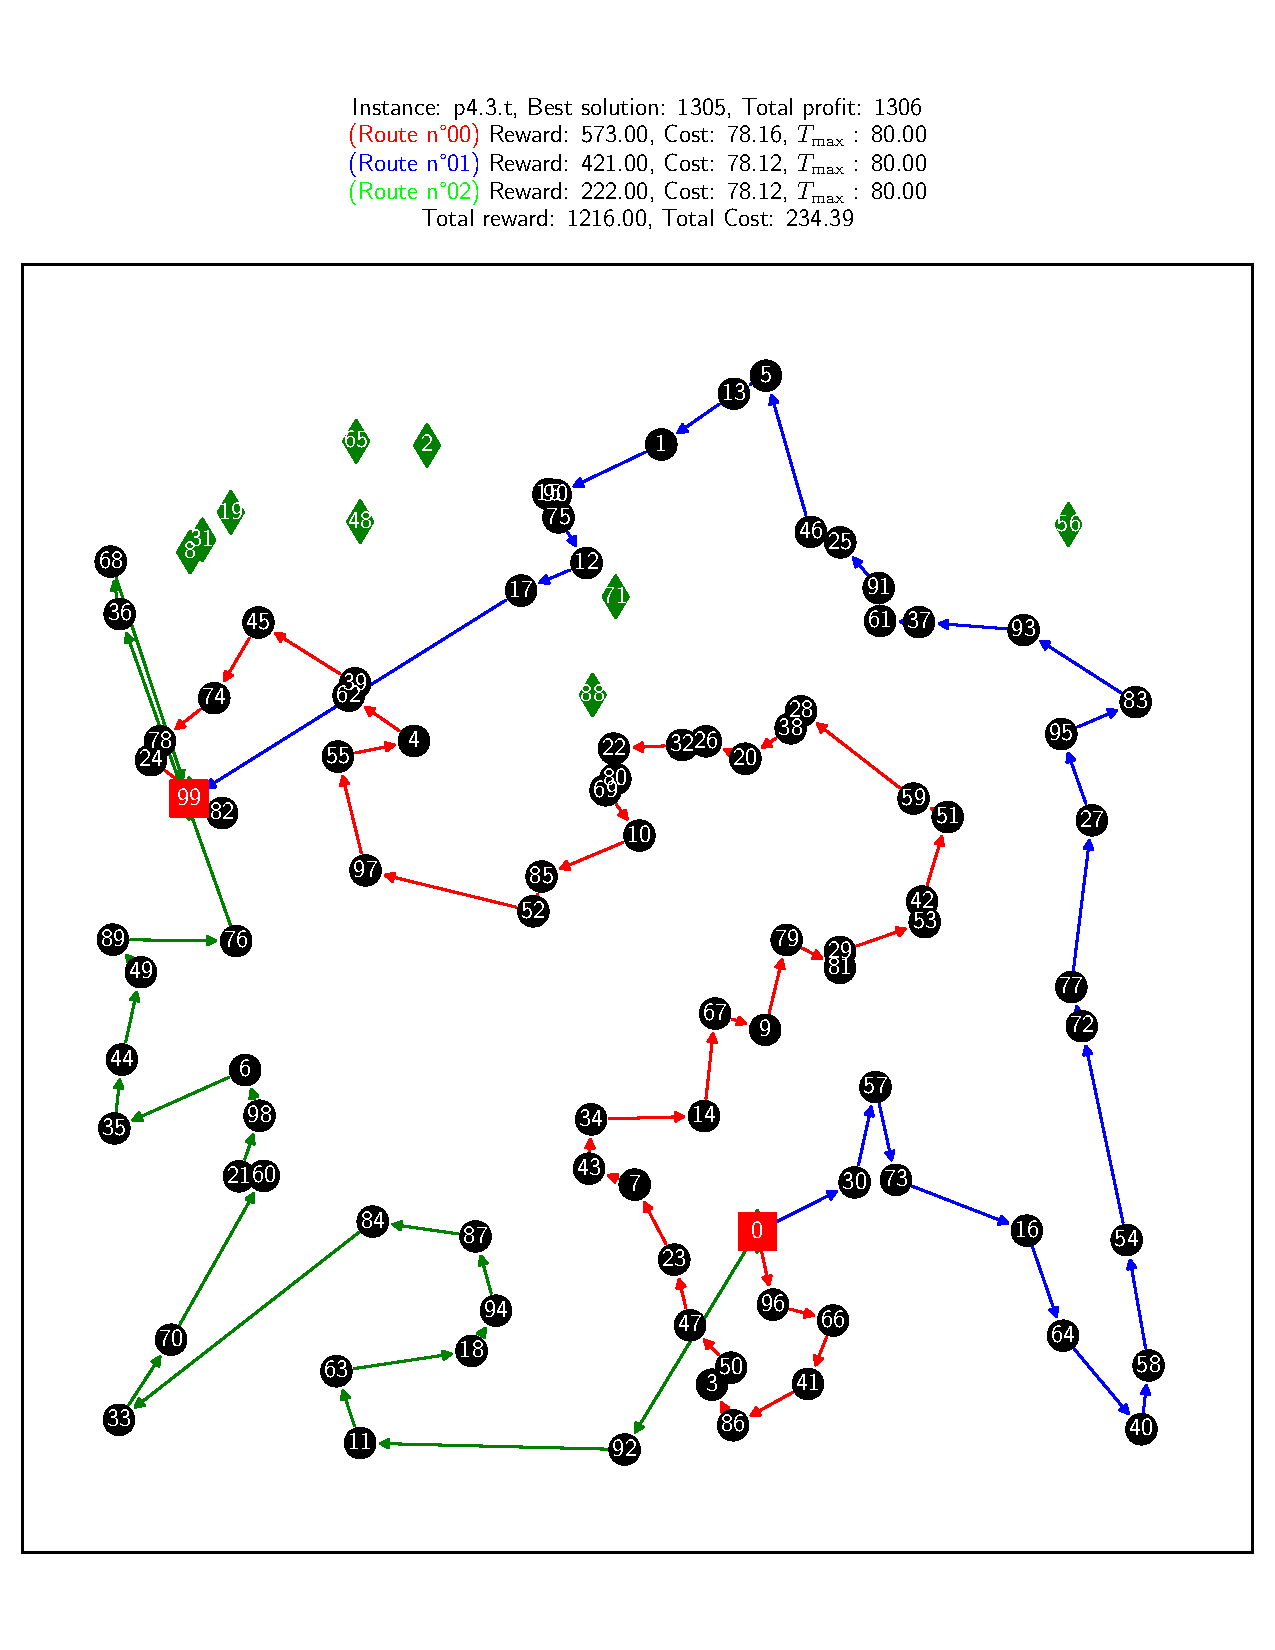
\includegraphics[width=\textwidth]{alns_p4.3.t.pdf}
	\caption{Solution proposée pour l'instance \textquote{p4.3.t}}
	\label{fig:alns}
\end{figure}


\printnoidxglossary[type=acronym]
\printbibliography

\end{document}
